% chapters/chapter2/2_8_wheels_force.tex
% !TeX root=../../main.tex

\section{محاسبه بارهای عمودی چرخ‌ها}
\label{sec:wheels_force}

پس از استخراج معادلات حرکت سیستم، ارزیابی نیروهای وارد بر تکیه‌گاه‌ها و بارهای عمودی چرخ‌های ارابه برای بررسی عملکرد دینامیکی سازه اهمیت می‌یابد. بارهای وارد بر چرخ‌ها از کمیت‌های مهم در ارزیابی بارگذاری و خستگی سازه مسیر جرثقیل محسوب می‌شوند \cite{Kettler2020WheelLoads}. هدف از این بخش، محاسبه نیروهای عمودی دو سمت ارابه با استفاده از شتاب‌های استخراج‌شده در مدل لاگرانژی است.

\subsection{فرضیات و مدل‌سازی هندسی}
برای تعیین بارهای عمودی، توزیع نیروها بر اساس هندسه ارابه و با در نظر گرفتن فرضیات زیر انجام می‌گیرد:
\begin{itemize}
    \item نیروی محرک $F$ در راستای افقی و هم‌راستا با مرکز جرم ارابه اعمال می‌شود؛ در نتیجه، گشتاور مستقیمی حول مرکز جرم ایجاد نمی‌کند.
    \item نقطه اتصال پاندول منطبق بر مرکز جرم ارابه در نظر گرفته شده است.
    \item جرم ارابه برابر $M$ و جرم بار نقطه‌ای برابر $m$ است.
    \item دو مجموعه چرخ از نظر عرضی نسبت به صفحه مدل متقارن فرض شده‌اند و در این مدل دوبعدی، هر کدام به صورت یک نیروی عمودی معادل $F_{w1}$ (تکیه‌گاه چپ) و $F_{w2}$ (تکیه‌گاه راست) با جهت مثبت رو به بالا تعریف می‌شوند.
    \item فاصله افقی محل تماس هر مجموعه چرخ تا مرکز جرم ارابه برابر $D_1$ است.
    \item محل تماس چرخ‌ها با ریل در راستای قائم به اندازه $D_2$ پایین‌تر از مرکز جرم ارابه قرار دارد.
    \item اثر اصطکاک لزج ارابه به صورت نیروی افقی $F_{bc} = b_c\dot{x}$ در محل تماس چرخ‌ها با ریل اعمال می‌شود.
    \item جرم چرخ‌ها و انعطاف‌پذیری سازه ارابه و ریل در این محاسبات لحاظ نشده‌اند.
\end{itemize}

شماتیک توزیع نیروها و هندسه ارابه در شکل \ref{fig:wheels_force} نشان داده شده است.

\begin{figure}[htbp]
    \centering
    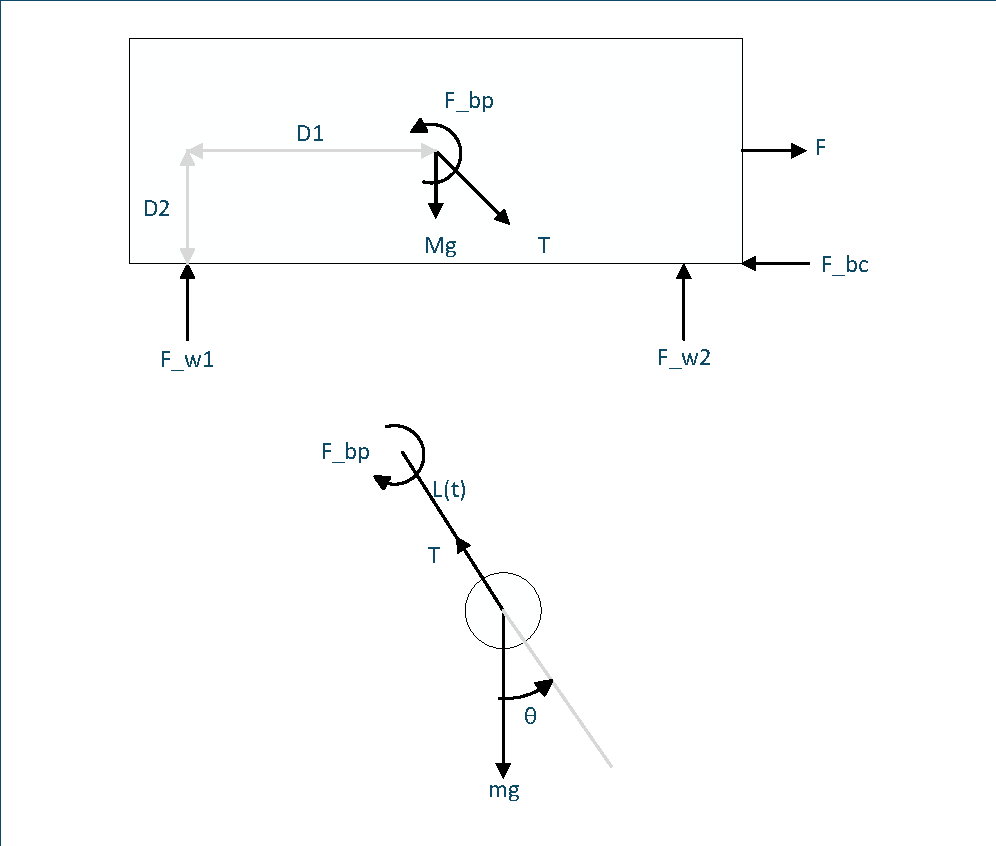
\includegraphics[width=0.9\textwidth]{images/0_System_Modeling/Wheels_Force.pdf}
    \caption{\rl{نیروها و هندسه مورد استفاده برای محاسبه بارهای عمودی وارد بر مجموعه چرخ‌های ارابه.}}
    \label{fig:wheels_force}
\end{figure}

\subsection{محاسبه سینماتیک و موازنه نیروها}
محاسبه بار چرخ‌ها در این بخش به عنوان یک لایه پس‌پردازش دینامیکی بر روی مدل موجود عمل می‌کند. به عبارت دیگر، نیازی به استخراج مجدد معادلات حرکت با روش نیوتن-اویلر نیست و شتاب‌های $\ddot{x}$ و $\ddot{\theta}$ مستقیماً از مدل دینامیکی غیرخطی (مبتنی بر روش لاگرانژ) دریافت می‌شوند.

ابتدا شتاب افقی و قائم بار آویخته با مشتق‌گیری از معادلات سینماتیکی، به صورت زیر به دست می‌آیند:
\begin{equation}
    \ddot{x}_p = \ddot{x} + \ddot{l}\sin\theta + 2\dot{l}\dot{\theta}\cos\theta + l\ddot{\theta}\cos\theta - l\dot{\theta}^2\sin\theta
\end{equation}
\begin{equation}
    \ddot{y}_p = -\ddot{l}\cos\theta + 2\dot{l}\dot{\theta}\sin\theta + l\ddot{\theta}\sin\theta + l\dot{\theta}^2\cos\theta
\end{equation}

با اعمال اصل دالامبر و موازنه نیروها در راستای قائم برای کل مجموعه ارابه و بار، مجموع بارهای عمودی چرخ‌ها ($F_\Sigma$) استخراج می‌شود:
\begin{equation}
    F_\Sigma = F_{w1} + F_{w2} = (M+m)g + m\ddot{y}_p
\end{equation}
رابطه فوق نشان می‌دهد که مجموع بار عمودی وارد بر ریل، برابر با وزن کل سیستم به علاوه مؤلفه دینامیکی ناشی از شتاب قائم بار است.

برای تعیین نحوه توزیع بار میان تکیه‌گاه‌های چپ و راست، موازنه گشتاور حول مرکز جرم ارابه صورت می‌گیرد. با استفاده از مختصات نسبی جرم بار نسبت به مرکز جرم ($x_r = l\sin\theta$ و $y_r = -l\cos\theta$) و لحاظ کردن گشتاورهای ناشی از اصطکاک ارابه، نیروی وزن بار و نیروی اینرسی آن، اختلاف بار چرخ‌ها ($F_\Delta$) به صورت فشرده زیر محاسبه می‌شود:
\begin{equation}
    F_\Delta = F_{w2} - F_{w1} = \frac{D_2 b_c \dot{x} + m g l \sin\theta + m\left( l\sin\theta\,\ddot{y}_p + l\cos\theta\,\ddot{x}_p \right)}{D_1}
\end{equation}

پس از استخراج مقادیر مجموع و اختلاف نیروها، بار عمودی هر یک از چرخ‌ها از طریق حل این دستگاه دو معادله‌ای مستقیماً محاسبه می‌گردد:
\begin{equation}
    F_{w1} = \frac{F_\Sigma - F_\Delta}{2}
\end{equation}
\begin{equation}
    F_{w2} = \frac{F_\Sigma + F_\Delta}{2}
\end{equation}

روند کلی این پس‌پردازش دینامیکی را می‌توان در زنجیره محاسباتی زیر خلاصه کرد:
\begin{equation*}
    \ddot{x}, \ddot{\theta} \quad \Rightarrow \quad \ddot{x}_p, \ddot{y}_p \quad \Rightarrow \quad F_\Sigma, F_\Delta \quad \Rightarrow \quad F_{w1}, F_{w2}
\end{equation*}

جزئیات محاسبات نمادین و راستی‌آزمایی این روابط، در اسکریپت کد \ref{code:wheels_force} از پیوست \ref{app:matlab_codes} ارائه شده است.

\subsection{بارگذاری دینامیکی چرخ‌ها به عنوان معیار ارزیابی}
هدف از استخراج روابط نیروهای $F_{w1}$ و $F_{w2}$ در این پژوهش، توسعه مدل سایش یا پیش‌بینی دقیق عمر خستگی نیست؛ بلکه این مقادیر به عنوان یک شاخص کمکی برای ارزیابی بارگذاری دینامیکی سیستم و مقایسه عملکرد کنترل‌کننده‌ها به کار می‌روند.

در ارزیابی‌های آتی، برای هر معماری کنترلی، مسیرهای حالت سیستم شامل موقعیت، سرعت و شتاب‌های ارابه و پاندول از محیط شبیه‌سازی دریافت شده و در معادلات این بخش جایگذاری می‌شوند. با این رویکرد، امکان رسم پروفایل زمانی بارهای عمودی چرخ‌ها فراهم می‌گردد. کاهش قله‌های بیشینه بار و سرکوب نوسانات متناوب در نمودار نیروهای چرخ، از منظر بارگذاری دینامیکی، نشان‌دهنده عملکرد مطلوب‌تر الگوریتم در کاهش تنش‌های وارد بر سازه جرثقیل است.